% !TEX root = ../main.tex
\chapter{IoT Brain} \label{ch:framework}

This chapter is going to give some informations about the design choice taken while implementing the approaches in \textbf{\autoref{ch:model}} and \textbf{\autoref{ch:diagnosis}}.
Implementation efforts were aimed at providing a further degree of scalability to the approach and leveraging cloud based technologies as well as reducing the technicality of the involved resource.
It will be presented a use case that shows the % TODO explain why this framework can help in spreading a EMS
\section{Fully integrated BMS}
Previous chapters defined a possible approach for diagnosing smart buildings, developed by IBM Research and it has been shown that such a method works as expected.
However such instruments needs to be integrated in a broader panorama of services that should be present in a Smart Building. Defining the term Smart Building is a challenging task and various organizations adopt their own definition. % TODO add definitions
What emerges is that a smart building has to be able to perceive the context it is in, being aware of its status and its occupants. Another key concept it is its ability to react, and adapt, autonoumsly to changes in the environment, possibly predicting and optimizing its behaviour in order to optimize occupants comfort and energy consumption.
IoT devices provide the context for a Smart Building. Commercial buildings are costantly monitored by IoT smart sensors and meters that provide a huge amount of data. Those data are stored and processed to extract useful information on the state of the building. % TODO chart how many sensors
Analytics provide the means that the building use to interpret the context and react in a correct way. For example, let a fault occour at a Fan Coil Unit (FCU) in a room. A smart building should be able to detect it, diagnose it, eventually issue a repair request to the manteinance service with a description of the fault. Then, upon arrival of the mainteinance worker, the building should be able to guide said worker through the building itself towards the location of the fault.

\section{Requirements}
In a Smart Building context it is important to understand what are the main goals that are to be achived by the deployment of such a system. What emerged from this thesis work is that a Smart Building IT infrastructure needs to be build upon a scalable framework that provides a platform for easy and fast analytics deployement. There's a need of a middleware that provide every top level application with a common ground that abstract the physical sensors so that the whole system is integrated and top layer components are able to exchange informations. % example integration of weather data etc.
This middleware is born from the Semantic Web concept of ontology (see \autoref{ch:semantic_web}) and of semantic reasoning.
On top of that it is important to identify the potential users of such a system. Those user are both those who benefit from the deployed analytics and those who are going to develop those analytics. It is important to note that none of those users is required to have a deep computer science background of any sort, still they are the ones with most interest in a smart building management system. The system should aim at providing those users the most straightforward default way to interact with the system, trough high-level languages and possibily human language interfaces (see \ref{}) but still allows for low level interaction where needed. To sum it up:
\begin{itemize}
  \item Easy development tools
  \item High level scripting languages
  \item Semantic capabilities to enable integration
  \item Scalable backend
\end{itemize}

\section{Knowledge Inference Technology for IoT}
Knowledge Inference Technology for IoT (KITT) is a layered framework that provide an API to model, manage and reason on the semantic knowledge of IoT Systems. It has been developed by IBM Research and expanded with further capabilities as the core of this thesis. It is designed to meet the requirements outlined in the previous section and to provide a service for integrated deployment of analytics in IoT contexts.
KITT adopt a layered approach as seen in \autoref{fig:kitt}.
\begin{figure}
  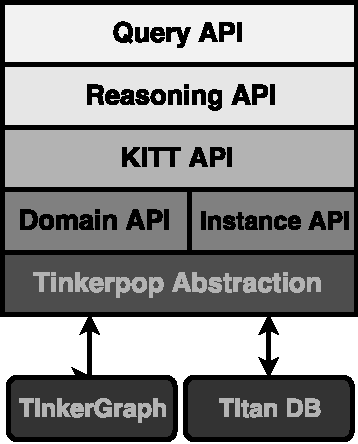
\includegraphics{kitt.pdf}
  \caption{KITT internal structure}
  \label{fig:kitt}
\end{figure}
Each of these layers implements different functionalities that will be detailed just below

\paragraph{TinkerPop Abstraction}
One of the main 


%IoT Big scale Reasoning and Analytic INsights (IoT BRAIN) allows to specify semantic models for IoT systems and run analytics across them automatically. Its core is the light-weight knowledge framework named Knowledge Inference Technology for IoT (KITT) that provides a simple API to model, manage and reason on the semantic knowledge model. It is split in multiple layers of different abstraction level that base on a common semantic modeling strategy.
%This architecture has been developed implements the concepts explained in the previous chapters with a strong emphasis on the scalability and availability of the approach.

\begin{figure}
  \centering
  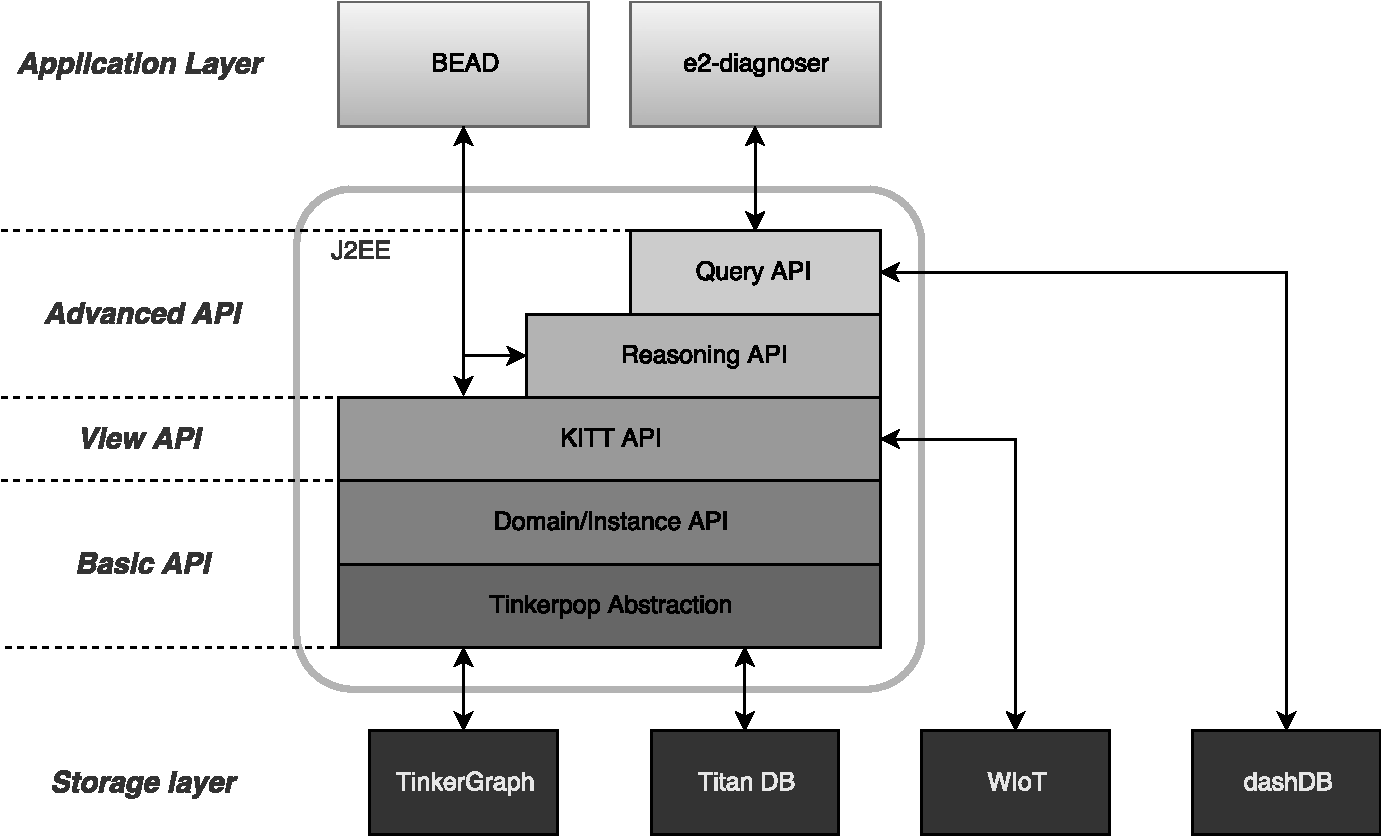
\includegraphics[width=1\textwidth]{iot_brain.pdf}
  \caption{IoT BRAIN architecture}
  \label{fig:iot_brain}
\end{figure}

%IoT BRAIN, which architecture is shown in \autoref{fig:iot_brain}, is built upon a storage layer that is comprised of a graph database, used for storing the semantic model of the building. The Watson IoT platform allows easy connection and dispatch of data securely to the cloud using the open, lightweight MQTT messaging protocol. The storage layer is completed by a dashDB, an SQL database that provides efficient storage of time series and high query performance. On top of this layer sits the core of the project which realize the theoric process shown in \autoref{fig:approach_overview}.
